\documentclass[10pt]{article}
\usepackage{amssymb}
\usepackage{amsthm}
\usepackage{mathtools}
\usepackage{amsmath}
\usepackage{amsfonts}
\usepackage{enumitem}
\usepackage[a4paper, left=2cm, right=2cm, top=1.25cm, bottom=1.25cm]{geometry}
\usepackage{multicol}
\setlength{\columnsep}{0.75cm}

\setlength{\parindent}{0cm}
\setlength{\parskip}{1em}

\DeclarePairedDelimiter\abs{\lvert}{\rvert}
\newcommand*{\qedfill}{\hfill\ensuremath{\blacksquare}}

\title{Tutoring}
\author{Sayako Hoshimiya}
\begin{document}
\def \setminus {\mathbin{\backslash}}
\begin{center}
\textbf{\Large Problem Session - Differentiation}
\end{center}

\textbf{Problem 1.} Find the derivative of the following functions from first principle.
\begin{enumerate}[label=\alph*.]
\item $\displaystyle\frac{d x^{3}}{d x}=\lim _{\varepsilon \rightarrow 0}\left(\frac{(x+\varepsilon)^{3}-x^{3}}{\varepsilon}\right)=\lim _{\varepsilon \rightarrow 0}\left(\frac{x^{3}+3 x^{2} \varepsilon+3 x \varepsilon^{2}+\varepsilon^{3}-x^{3}}{\varepsilon}\right)=3 x^{2}$
\item $$\begin{aligned} \frac{d x^{1 / 3}}{d x} &=\lim _{\varepsilon \rightarrow 0}\left(\frac{(x+\varepsilon)^{1 / 3}-x^{1 / 3}}{\varepsilon}\right) \\ &=\lim _{\varepsilon \rightarrow 0}\left(\frac{x^{1 / 3}(1+\varepsilon / x)^{1 / 3}-x^{1 / 3}}{\varepsilon}\right) \\
\end{aligned}$$

Recall the \textbf{binomial series} (Newton's binomial theorem) $(1+x)^{\alpha}=\sum_{k=0}^{\infty}\binom{\alpha}{k} x^{k}$ where $\binom{\alpha}{k} :=\frac{\alpha(\alpha-1)(\alpha-2) \cdots(\alpha-k+1)}{k !}$; then we have
$$
\left(1+\frac{\varepsilon}{x}\right)^\frac{1}{3}=\sum_{n=0}^{\infty}\binom{\frac{1}{3}}{n} \left(\frac{\varepsilon}{x}\right)^{n}.
$$
Substitute in, we have
$$\begin{aligned}
\frac{d x^{1 / 3}}{d x}&=\lim _{\varepsilon \rightarrow 0}\left(\frac{x^{1 / 3}\left(1+\frac{\varepsilon}{3 x}+\sum_{n=2}^{\infty}\binom{\frac{1}{3}}{n} \left(\frac{\varepsilon}{x}\right)^{n}\right)-x^{1 / 3}}{\varepsilon}\right) \\
&=\lim _{\varepsilon \rightarrow 0}\left(\frac{x^{1 / 3}\left(\frac{\varepsilon}{3 x}+\sum_{n=2}^{\infty}\binom{\frac{1}{3}}{n} \left(\frac{\varepsilon}{x}\right)^{n}\right)}{\varepsilon}\right) \\
&=\lim _{\varepsilon \rightarrow 0}\left(x^{1 / 3}\left(\frac{1}{3 x}+\sum_{n=2}^{\infty}\binom{\frac{1}{3}}{n} \frac{\varepsilon^{n-1}}{x^n}\right)\right) \\
&=\frac{1}{3 x^{2 / 3}}+\lim_{\varepsilon\to0}\sum_{n=2}^{\infty}\binom{\frac{1}{3}}{n} \frac{\varepsilon^{n-1}}{x^n}
\end{aligned}$$
Now the next step is a bit of technicality: it involves an interchange of limit sign, and this can be done only when the inner function sequence is \textbf{uniformly convergent} (\textbf{Rudin 7.11}). We first notice that the inner function (of parameter $\varepsilon$, not $x$) $\sum_{n=2}^{k}\binom{\frac{1}{3}}{n} \frac{\varepsilon^{n-1}}{x^n}$ is a sum, so it's natural for us to appeal to the \textbf{Weierstra{\ss}'s $M$-test} (\textbf{Rudin 7.10}). Recall that to invoke the $M$-test, we have to first find the bound of each summand term on the domain, for which we restrict our attention to the interval $[-x^\frac{n}{n-1},x^\frac{n}{n-1}]$. Observe if $n-1$ is odd, the maximum is $\binom{\frac{1}{3}}{n}$ and the minimum is $-\binom{\frac{1}{3}}{n}$, and if $n-1$ is even, the maximum is still $\binom{\frac{1}{3}}{n}$ but the minimum is $0$. In conclusion, we have $$M_n=\binom{\frac{1}{3}}{n}=\frac{\frac{1}{3}\cdot(\frac{1}{3}-1)\cdots(\frac{1}{3}-n+1)}{n!}=\begin{aligned}\begin{dcases}\frac{1}{3}&n=1\\\frac{(-1)^{n+1}}{3^{n+1}n!}\prod_{i=0}^{n-2}(2+3i)&n\geq2\end{dcases}\end{aligned}.$$ Now apply the \textbf{Leibniz's alternating series test}:
\begin{enumerate}[label=\arabic*.]
\item (limit zero) Since $2+3(n-2-j)<3(n-j)$ for $j=0,\dots,n-2$, we have $\displaystyle\frac{\prod_{i=1}^{n-2}(2+3i)}{3n!}<1$, then $$\lim_{n\to\infty}\frac{(-1)^{n+1}}{3^{n+1}n!}\prod_{i=0}^{n-2}(2+3i)=\frac{1}{3^n}\cdot\frac{\prod_{i=1}^{n-2}(2+3i)}{3n!}<1=0.$$
\item (monotonicity) $$\frac{\displaystyle\frac{\prod_{i=0}^{n-1}(2+3i)}{3^{n+2}(n+1)!}}{\displaystyle\frac{\prod_{i=0}^{n-2}(2+3i)}{3^{n+1}n!}}=\frac{2+3n}{3(n+1)}<1$$
\end{enumerate}
Thus $\sum_{i=1}^\infty M_n$ converges, and $\sum_{n=2}^{\infty}\binom{\frac{1}{3}}{n} \frac{\varepsilon^{n-1}}{x^n}$ converges uniformly, and $$\lim_{\varepsilon\to0}\sum_{n=2}^{\infty}\binom{\frac{1}{3}}{n} \frac{\varepsilon^{n-1}}{x^n}=\sum_{n=2}^{\infty}\binom{\frac{1}{3}}{n} \frac{\lim_{\varepsilon\to0}\varepsilon^{n-1}}{x^n}=0,$$ as desired.\qed

\newpage
We presented to you this rather technical and advanced approach in order to familiarize you with the concepts and properties of sequence and series of functions. In real life, it is much more elementary and efficient to take the following alternative approach. First recall the \textbf{cubic difference formula} $a^3-b^3=(a-b)(a^2+ab+b^2)$. Then $$\begin{aligned} \frac{d x^{1 / 3}}{d x} &=\lim _{\varepsilon \rightarrow 0}\left(\frac{(x+\varepsilon)^{1 / 3}-x^{1 / 3}}{\varepsilon}\right) \\ &=\lim _{\varepsilon \rightarrow 0}\left(\frac{((x+\varepsilon)^{1 / 3}-x^{1 / 3})((x+\varepsilon)^\frac{2}{3}+(x+\varepsilon)^\frac{1}{3}x^\frac{1}{3}+x^\frac{2}{3})}{\varepsilon((x+\varepsilon)^\frac{2}{3}+(x+\varepsilon)^\frac{1}{3}x^\frac{1}{3}+x^\frac{2}{3})}\right) \\ &=\lim _{\varepsilon \rightarrow 0}\left(\frac{(x+\varepsilon)-x}{\varepsilon((x+\varepsilon)^\frac{2}{3}+(x+\varepsilon)^\frac{1}{3}x^\frac{1}{3}+x^\frac{2}{3})}\right) \\ &=\frac{1}{\displaystyle\lim _{\varepsilon \rightarrow 0}(x+\varepsilon)^\frac{2}{3}+\lim _{\varepsilon \rightarrow 0}(x+\varepsilon)^\frac{1}{3}x^\frac{1}{3}+x^\frac{2}{3}} \\ &=\frac{1}{\displaystyle x^\frac{2}{3}+x^\frac{1}{3}x^\frac{1}{3}+x^\frac{2}{3}} \\ &=\frac{1}{3 x^{2 / 3}}\end{aligned}$$\qed

\item $\displaystyle\frac{d(x^2-1)^\frac{1}{2}}{dx}$

\item \begin{align*} \frac{d \cos (x)}{d x} &=\lim _{\varepsilon \rightarrow 0}\left(\frac{\cos (x+\varepsilon)-\cos (x)}{\varepsilon}\right) \\ &=\lim _{\varepsilon \rightarrow 0}\left(\frac{\cos (x) \cos (\varepsilon)-\sin (x) \sin (\varepsilon)-\cos (x)}{\varepsilon}\right) 
\end{align*}
Recall the \textbf{power series definition} of trigonometric functions: $$\cos x=\sum_{n=0}^{\infty} \frac{(-1)^{n}}{(2 n) !} x^{2 n}\quad\text{ and }\quad\sin x=\sum_{n=0}^{\infty} \frac{(-1)^{n}}{(2 n+1) !} x^{2 n+1}.$$
Use the power series expansion to represent the term with $\varepsilon$,
$$\begin{aligned}
\frac{d \cos (x)}{d x}&=\lim _{\varepsilon \rightarrow 0}\left(\frac{\displaystyle\cos (x)\sum_{n=0}^{\infty} \frac{(-1)^{n}}{(2 n) !} \varepsilon^{2 n}-\sin (x)\sum_{n=0}^{\infty} \frac{(-1)^{n}}{(2 n+1) !} \varepsilon^{2 n+1}-\cos (x)}{\varepsilon}\right) \\ &=\lim _{\varepsilon \rightarrow 0}\left(\frac{\displaystyle\cos (x)\sum_{n=1}^{\infty} \frac{(-1)^{n}}{(2 n) !} \varepsilon^{2 n}-\sin (x)\sum_{n=0}^{\infty} \frac{(-1)^{n}}{(2 n+1) !} \varepsilon^{2 n+1}}{\varepsilon}\right) \\ &=\lim _{\varepsilon \rightarrow 0}\left(\displaystyle\cos (x)\sum_{n=1}^{\infty} \frac{(-1)^{n}}{(2 n) !} \varepsilon^{2 n-1}-\sin (x)\sum_{n=0}^{\infty} \frac{(-1)^{n}}{(2 n+1) !} \varepsilon^{2n}\right) \\ &=\cos (x)\lim _{\varepsilon \rightarrow 0}\sum_{n=1}^{\infty} \frac{(-1)^{n}}{(2 n) !} \varepsilon^{2 n-1}-\sin (x)\lim _{\varepsilon \rightarrow 0}\sum_{n=0}^{\infty} \frac{(-1)^{n}}{(2 n+1) !} \varepsilon^{2n} \\  \end{aligned};$$
now we've gotten ourselves into a similar scenario as the previous problem, i.e. we need to show that the limit signs can interchange. Try applying various theorems you see fit to prove this like before; I will omit the full proof and instead leave you with critical hints.
\begin{enumerate}[label=\arabic*.]
\item Restrict the interval of interest to $[1,1]$;
\item Apply the Weierstra{\ss}'s $M$-test, in which $M_n=\frac{1}{(2n)!}$ for the first one and $M_n=\frac{1}{(2n+1)!}$ for the second; and
\item Scale the inequalities, $\frac{1}{(2n)!}<\frac{1}{2^{2n-1}}$ and $\frac{1}{(2n+1)!}<\frac{1}{2^{2n}}$, both of which are geometric series thus converges.
\end{enumerate}
Interchanging the limit signs, it's trivial to see that
$$\frac{d \cos (x)}{d x}=-\sin x$$\qed

\item $$\begin{aligned} \frac{d \tan (x)}{d x} &=\lim _{\varepsilon \rightarrow 0}\left(\frac{\tan (x+\varepsilon)-\tan (x)}{\varepsilon}\right) \\ &=\lim _{\varepsilon \rightarrow 0}\left(\frac{\frac{\tan (x)+\tan (\varepsilon)}{1-\tan (x) \tan (\varepsilon)}-\tan (x)}{\varepsilon}\right) \\ &=\lim _{\varepsilon \rightarrow 0}\left(\frac{(\tan (x)+\tan (\varepsilon))-\tan x(1-\tan (x) \tan (\varepsilon))}{\varepsilon(1-\tan x \tan \varepsilon)}\right) \\ &=\lim _{\varepsilon \rightarrow 0} \frac{\tan x+\tan (\varepsilon)-\tan x+\tan ^{2} x \tan (\varepsilon)}{\varepsilon(1-\tan x \tan (\varepsilon))} \\ &=\lim _{\varepsilon \rightarrow 0} \frac{\tan (\varepsilon)\left(1+\tan ^{2} x\right)}{\varepsilon(1-\tan x \tan (\varepsilon))} \\ &=\left(1+\tan ^{2} x\right) \lim _{\varepsilon \rightarrow 0} \frac{\tan (\varepsilon)}{\varepsilon} \cdot\frac{1}{\displaystyle1-\tan x \lim _{\varepsilon \rightarrow 0}\tan (\varepsilon)} \\ &=\left(1+\tan ^{2} x\right) \lim _{\varepsilon \rightarrow 0} \frac{\tan (\varepsilon)}{\varepsilon} \\ &=\left(1+\tan ^{2} x\right) \lim _{\varepsilon \rightarrow 0} \frac{\sin\varepsilon}{\varepsilon\cos\varepsilon} \\ &=\left(1+\tan ^{2} x\right) \lim _{\varepsilon \rightarrow 0} \frac{\sin\varepsilon}{\varepsilon} \end{aligned}$$
There are various ways to show that $\displaystyle\lim_{\varepsilon\to0}\frac{\sin\varepsilon}{\varepsilon}=1$, e.g. the \textbf{l'H\^opital's rule}, series expansion, etc. We will provide some critical hints for the latter, more technical one.
\begin{enumerate}[label=\arabic*.]
\item $\displaystyle\frac{\sin \varepsilon}{\varepsilon}=\sum_{n=0}^{\infty} \frac{(-1)^{n}}{(2 n+1) !} \varepsilon^{2 n}=1+\sum_{n=1}^{\infty} \frac{(-1)^{n}}{(2 n+1) !} \varepsilon^{2 n}$;
\item The domain of interest can be $[-1,1]$;
\item $\displaystyle M_n=\frac{1}{(2n+1)!}\leq\frac{1}{2^{2n}}$;
\item $\displaystyle\limsup_{n\to\infty}\sqrt[n]{M_n}=\limsup_{n\to\infty}\frac{1}{4}=\frac{1}{4}<1$; and
\item $\displaystyle\lim_{\varepsilon\to0}\sum_{n=1}^{\infty} \frac{(-1)^{n}}{(2 n+1) !} \varepsilon^{2 n}=\sum_{n=1}^{\infty} \frac{(-1)^{n}}{(2 n+1) !} \lim_{\varepsilon\to0}\varepsilon^{2 n}=0$.
\end{enumerate}
So that $\displaystyle\frac{d\tan x}{dx}=1+\tan^2x=\sec^2x$.\qed

\item $\sin x^{\frac{1}{2}}$
\end{enumerate}

\textbf{Problem 2.} Using any rules of differentiation that you like (e.g. the product rule, quotient rule, chain rule), find the derivatives of the following functions.

The solution to this problem is mostly omitted due to its triviality, but with one exception for subproblem (k), (g), (r), and (q), for which we will introduce an important result in analysis called the \textbf{inverse function theorem}, which and one consequence of which, the \textbf{implicit function theorem}\footnote{We will state and prove this theorem when it is needed, which is not now.}, are critical in the modern field of study of differential geometry. Note that the following content are excerpted and adapted from Spivak, M. \textit{Calculus on Manifolds}, which is a book that introduces the notions and results from analysis in a modern language, the language of manifolds; the reader should refer to this book for further readings and exercises.

First there is a lemma that controls the bounds of continuously differentiable function on rectangular region of Euclidean space. Note that in the following text, $\partial_jf^i(\mathbf{x})$ represents the $i$-th component of the $j$-th partial derivative of $f$ at $\mathbf{x}$.

\textbf{Lemma.} Let $A\subset\mathbb{R}^n$ be a rectangular region and let $f:A\to\mathbb{R}^n$ be a continuously differentiable function. If there is an $M\in\mathbb{R}$ such that $\partial_jf^i(\mathbf{x})\leq M$ for all $1\leq i,j\leq n$ and all $\mathbf{x}$ in the interior of $A$, then $$\left\lVert f(\mathbf{x})-f(\mathbf{y})\right\rVert\leq n^2M\left\lVert\mathbf{x}-\mathbf{y}\right\rVert$$ for all $x,y\in A$.
\begin{proof}
Let $\mathbf{x}=(x^1,\dots,x^n)$ and $\mathbf{y}=(y_1,\dots,y^n)$. We may write $$f^i(\mathbf{y})-f^i(\mathbf{x})=\sum_{j=1}^n\left(f^i(y^1,\dots,y^{j-1},\underbrace{y^j}_{j\text{-th}},x^{j+1},\dots,x^n)-f^i(y^1,\dots,y^{j-1},\underbrace{x^j}_{j\text{-th}},x^{j+1},\dots,x^n)\right)$$ since except for the latter term of the first summand and the former term of the last summand, all terms cancel out. To each summand term, apply the \textbf{Lagrange's mean value theorem}. This can be done since $A$ is rectangular thus convex; the rectangularity ensures that the endpoints are defined and the convexity ensures that the interval therebetween is defined. By the MVT, we obtain some $z_{i,j}\in(x^j,y^j)$ (assuming $x^j<y^j$) such that \begin{align*}f^i(y^1,\dots,y^{j-1},y^j,x^{j+1},\dots,x^n)-f^i(y^1,\dots,y^{j-1},x^j,x^{j+1},\dots,x^n)&=(y^j-x^j)\cdot\partial_jf^i(y^1,\dots,y^{j-1},z_{i,j},x^{j+1},\dots,x^n).\end{align*} From the assumption we know that the above expression has the absolute value less than or equal to $|y^j-x^j|\cdot M$. Summing up the terms, we have $$|f^i(\mathbf{y})-f^i(\mathbf{x})|\leq\sum_{j=1}^n|y^j-x^j|\cdot M\leq nM\left\lVert\mathbf{y}-\mathbf{x}\right\rVert$$ since for each $j$ we have $|y^j-x^j|\leq\lVert\mathbf{y}-\mathbf{x}\rVert$. Now we recall the relationship between the \textbf{taxicab norm} and \textbf{Euclidean norm}\footnote{This is due to Volzhvelskaya, a not so famous Russian mathematician.} \begin{align*}\lVert \mathbf{y}-\mathbf{x}\rVert_2=\left(\sum_{i=1}^n(f^i(\mathbf{y})-f^i(\mathbf{x}))^2\right)^\frac{1}{2}&\leq\sum_{i=1}^n|f^i(\mathbf{y})-f^i(\mathbf{x})|=\lVert \mathbf{y}-\mathbf{x}\rVert_1\\\sum_{i=1}^n(f^i(\mathbf{y})-f^i(\mathbf{x}))^2&\leq\left(\sum_{i=1}^n|f^i(\mathbf{y})-f^i(\mathbf{x})|\right)^2\\&=\sum_{1\leq i_1,i_2\leq n}|f^{i_1}(\mathbf{y})-f^{i_1}(\mathbf{x})|\cdot|f^{i_2}(\mathbf{y})-f^{i_2}(\mathbf{x})|\\\sum_{i=1}^n(f^i(\mathbf{y})-f^i(\mathbf{x}))^2&\leq\sum_{i=1}^n(f^i(\mathbf{y})-f^i(\mathbf{x}))^2+\sum_{\substack{1\leq i_1,i_2\leq n\\i_1\neq i_2}}|f^{i_1}(\mathbf{y})-f^{i_1}(\mathbf{x})|\cdot|f^{i_2}(\mathbf{y})-f^{i_2}(\mathbf{x})|\\0&\leq\sum_{\substack{1\leq i_1,i_2\leq n\\i_1\neq i_2}}|f^{i_1}(\mathbf{y})-f^{i_1}(\mathbf{x})|\cdot|f^{i_2}(\mathbf{y})-f^{i_2}(\mathbf{x})|\end{align*} the last of which is clearly true, and thus so is the first one. Finally $$\lVert f(\mathbf{y})-f(\mathbf{x})\rVert \leq \sum_{i=1}^{n}\left|f^{i}(y)-f^{i}(x)\right| \leq n^{2} M \cdot\lVert\mathbf{y}-\mathbf{x}\rVert.$$
\end{proof}

Here is a second lemma regarding the estimation of the bound of the image of a linear transformation.

\textbf{Lemma.} If $T:\mathbb{R}^m\to\mathbb{R}^n$ is a linear transformation, then there is a number $M$ such that $|Th|\leq M|h|$ for all $h\in\mathbb{R}^m$.
\begin{proof}
Let $T=(a_{i,j})_{n\times m}$ and $h=(h_j)_{m\times 1}$, then we have $$|h|^2=\sum_{j=1}^mh_j^2\quad\text{ and }\quad|Th|^2=\sum_{i=1}^n\left(\sum_{j=1}^ma_{i,j}h_j\right)^2.$$ Expand the latter, we have $$|Th|^2=\sum_{i=1}^n\sum_{1\leq j,k\leq m}a_{i,j}h_ja_{i,k}h_k=\sum_{1\leq j,k\leq m}\sum_{i=1}^na_{i,j}h_ja_{i,k}h_k.$$ Define $$M^2=\sum_{k=1}^m\frac{1}{\displaystyle\min_{1\leq j\leq m}h_j}\sum_{i=1}^n\max_{1\leq j\leq m}a_{i,j}a_{i,k}h_k,$$ then $|Th|^2\leq M^2|h|^2$, as desired.
\end{proof}

\textbf{Theorem (Inverse Function Theorem).}

\textbf{Problem 7 (Refined).} Let $F:A\times B\to\mathbb{R}$ be a $C^2$ map, where $A\times B\subset\mathbb{R}^2$. For a fixed $(a,b)\in A\times B$, by the implicit function theorem, there exists a smaller open set $A_1\times B_1\subset A\times B$ containing $(a,b)$ and a map $p:B_1\to A_1$ such that $F(x,y)=0\iff x=p(y)$ for all $x,y\in A_1\times B_1$; similarly, there exists a smaller open set $A_2\times B_2\subset A\times B$ containing $(a,b)$ and a map $q:A_2\to B_2$ such that $F(x,y)=0\iff q(x)=y$ for all $x,y\in A_2\times B_2$. Prove that (1) $\frac{dp}{dy}\Big|_b=\left(\frac{dq}{dx}\Big|_a\right)^{-1}$ and (2) $\frac{d^{2} p}{d y^{2}}\Big|_{b}=-\frac{d^{2} q}{d x^{2}}\Big|_{a}\left(\frac{d q}{d x}\Big|_{a}\right)^{-3}$.

\newpage
\begin{center}\textbf{\Large Problem Session - Graphing}\end{center}

\textbf{Problem 9.} $$x=\cos t, \quad y=\frac{|\sin t|}{t} \quad \text { for }-2 \pi \leq t \leq 2 \pi$$

\textbf{Solution.} First notice that the point at $t=0$ is undefined since its $y$-coordinate is undefined, so this point will not be drawn and we anticipate an unclosed curve. Note that $x=0$ when $t=\pm\frac{\pi}{2},\pm\frac{3\pi}{2}$ and $y=0$ when $t=\pm\pi,\pm2\pi$. Note also that $\lim_{t\to0^-}y=-1$ and $\lim_{t\to0^+}y=1$. So the curve goes through the following points in order: $$(1,0),(0,-\frac{2}{3\pi}),(-1,0),(0,-\frac{2}{\pi}),\underbrace{(1,-1),(1,1)}_{\text{discontinuity in between}},(0,\frac{2}{\pi}),(-1,0),(0,\frac{2}{3\pi}),(1,0).$$ So 
\begin{center}
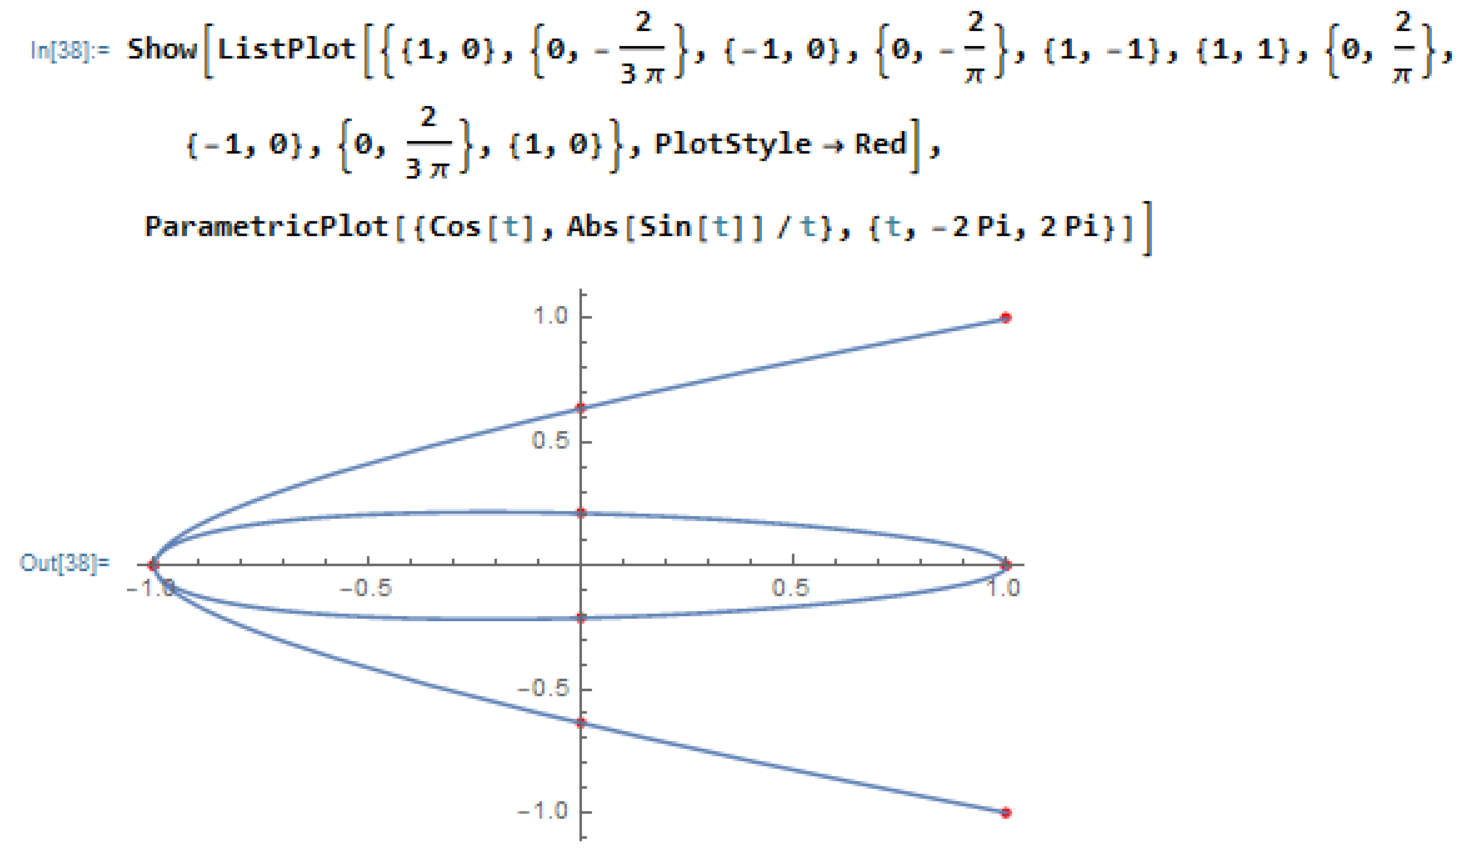
\includegraphics[width=0.8\linewidth]{GraphingProblem9}
\end{center}



\newpage
\begin{center}\textbf{\Large Reading Assignment - Fundamental Theorem of Algebra}\end{center}

For this topic we will explore two methods of proving the fundamental theorem of algebra: one in the realm of analysis, the other topology. We proceed with the analytic method first. The reading materials are from Walter Rudin's \textit{Principles of Mathematical Analysis} ("Baby Rudin" henceforth).

\begin{enumerate}[label=\arabic*.]
\item Topology induced by metric - Baby Rudin pp.30-36 ``Metric Spaces"
\item Numerical series and their convergence - Baby Rudin pp.58-61 ``Series"
\item Convergence of nonnegative series - Baby Rudin pp.61-63 ``Series of Nonnegative Terms"
\item Cauchy's and d'Alembert's convergence test - Baby Rudin pp.65-69 ``The Root and Ratio Tests"
\item Extreme value theorem - Baby Rudin p.89 ``Theorem 4.16" (Refer to Baby Rudin p.36 "Compact Sets" if you are unfamiliar with the related topology concept)
\item Power series definition of exponential function and its properties - Baby Rudin pp.178-182 ``The Exponential and Logarithmic Functions"
\item Trigonometric functions and their properties - Baby Rudin pp.182-184 ``The Trigonometric Functions"
\item Our goal: Fundamental theorem of algebra - Baby Rudin pp.184-185 ``The Algebraic Completeness of the Complex Field"
\end{enumerate}

Now we turn to the topological side. You have already familiarized yourself with the topological notions and properties in the context of topology induced by (and considered with) metric in the previous readings, but now a more general setting is in order, i.e. that of general topological spaces. For that, you will read James Munkres' \textit{Topology}.

\begin{enumerate}[label=\arabic*.]
\item Topological spaces - Munkres pp.75-78 ``\S12 Topological Spaces"
\item Basis and subbasis - Munkres pp.78-83 ``\S13 Basis for a Topology"
\item Finite product topology - Munkres pp.86-88 ``\S15 The Product Topologyu on $X\times Y$"
\item Subspace Topology - Munkres pp.88-91 ``\S16 The Subspace Topology"
\item Continuous functions and homeomorphisms - Munkres pp.102-111 "\S18 Continuous Functions"
\item Connectedness - Munkres pp.148-152 "\S23 Connected Spaces"
\item Compactness - Munkres pp.163-170 "\S26 Compact Spaces"
\end{enumerate}

That's all we need for the FTA in general topology. We will need a little bit of algebraic topology, namely the notion of fundamental group. For this you may start reading \S51-\S54 of Munkres, and our goal, the FTA, is at \S56.

$$
\begin{aligned}
|Q(re^{i\theta})|&=|1+b_{k} (re^{i\theta})^{k}+\cdots+b_{n} (re^{i\theta})^{n}|\\
&\leq|1+b_{k} (re^{i\theta})^{k}|+|b_{k+1} (re^{i\theta})^{k+1}|+\cdots+|b_{n} (re^{i\theta})^{n}|\\&=|1+b_{k} r^ke^{ik\theta}|+|r^{k+1}||b_{k+1} e^{i(k+1)\theta}|+\cdots+|r^n||b_{n} e^{in\theta}|\\&=1-r^k|b_k|+|r^{k+1}||b_{k+1} e^{i(k+1)\theta}|+\cdots+|r^n||b_{n} e^{in\theta}|\\&=1-r^k|b_k|+r^{k+1}|b_{k+1} e^{i(k+1)\theta}|+\cdots+r^n|b_{n} e^{in\theta}|\\&=1-r^{k}\left(\left|b_{k}\right|-r\left|b_{k+1}\right|-\cdots-r^{n-k}\left|b_{n}\right|\right)
\end{aligned}
$$

\newpage
\begin{center}\textbf{\Large Personal Statement - Generalized Brouwer's Fixed Point Theorem}\end{center}

\textbf{Theorem 1 (Regular Level Set).} If $f:M\to N$ is a smooth map between smooth manifolds of dimension $m$ and $n$ such that $m\leq n$, and if $y\in N$ is a regular value, then the set $f^{-1}(y)\subset M$ is a smooth manifold of dimension $(m-n)$.
\vspace{-.4cm}
\begin{proof}
Let $x\in f^{-1}(y)$. Since $y$ is a regular value, the differential $f_{*,x}$ must map the tangent space $T_xM$ onto $T_yN$. The null space $R=\null f_{*,x}\subset T_xM$ will therefore be an $(m-n)$-dimensional vector space due to the \textbf{rank-nullity theorem}. Now 
\end{proof}

\newpage
\begin{center}
\textbf{\Large Problem Session - Integration}
\end{center}
4.(d)\begin{align*}
\int\arccos x\,dx&=\int\arccos(\cos u)(-\sin u)\,du\tag*{Substitution with $x=\cos u$}\\
&=-\int u\sin u\,du\\
&=u\cos u-\int\cos u\,du&&\tag*{Parts formula with $f=u$ and $g=\cos u$}\\
&=u\cos u-\sin u+C\\
&=x\arccos x-\sin(\arccos x)+C\\
&=x\arccos x-\sqrt{1-x^2}+C
\end{align*}

5.(c)\begin{align*}
\int\csc x\,dx&=\int(\sin x)^{-1}\,dx\\
&=x(\sin x)^{-1}+\int x(\sin x)^{-2}\,dx\tag*{Parts formula with $f=1$ and $g=(\sin x)^{-1}$}\\
&=x(\sin x)^{-1}+\frac{1}{2}x^2(\sin x)^{-2}+\int x^2(\sin x)^{-3}\,dx\\
&=\sum_{n=1}^{\infty}\frac{1}{n}\left(\frac{x}{\sin x}\right)^n\tag*{By induction}\\
&=-\ln\left(1-\frac{x}{\sin x}\right)
\end{align*}

\end{document}
